% Options for packages loaded elsewhere
% Options for packages loaded elsewhere
\PassOptionsToPackage{unicode}{hyperref}
\PassOptionsToPackage{hyphens}{url}
\PassOptionsToPackage{dvipsnames,svgnames,x11names}{xcolor}
%
\documentclass[
  letterpaper,
  DIV=11,
  numbers=noendperiod]{scrartcl}
\usepackage{xcolor}
\usepackage{amsmath,amssymb}
\setcounter{secnumdepth}{5}
\usepackage{iftex}
\ifPDFTeX
  \usepackage[T1]{fontenc}
  \usepackage[utf8]{inputenc}
  \usepackage{textcomp} % provide euro and other symbols
\else % if luatex or xetex
  \usepackage{unicode-math} % this also loads fontspec
  \defaultfontfeatures{Scale=MatchLowercase}
  \defaultfontfeatures[\rmfamily]{Ligatures=TeX,Scale=1}
\fi
\usepackage{lmodern}
\ifPDFTeX\else
  % xetex/luatex font selection
\fi
% Use upquote if available, for straight quotes in verbatim environments
\IfFileExists{upquote.sty}{\usepackage{upquote}}{}
\IfFileExists{microtype.sty}{% use microtype if available
  \usepackage[]{microtype}
  \UseMicrotypeSet[protrusion]{basicmath} % disable protrusion for tt fonts
}{}
\makeatletter
\@ifundefined{KOMAClassName}{% if non-KOMA class
  \IfFileExists{parskip.sty}{%
    \usepackage{parskip}
  }{% else
    \setlength{\parindent}{0pt}
    \setlength{\parskip}{6pt plus 2pt minus 1pt}}
}{% if KOMA class
  \KOMAoptions{parskip=half}}
\makeatother
% Make \paragraph and \subparagraph free-standing
\makeatletter
\ifx\paragraph\undefined\else
  \let\oldparagraph\paragraph
  \renewcommand{\paragraph}{
    \@ifstar
      \xxxParagraphStar
      \xxxParagraphNoStar
  }
  \newcommand{\xxxParagraphStar}[1]{\oldparagraph*{#1}\mbox{}}
  \newcommand{\xxxParagraphNoStar}[1]{\oldparagraph{#1}\mbox{}}
\fi
\ifx\subparagraph\undefined\else
  \let\oldsubparagraph\subparagraph
  \renewcommand{\subparagraph}{
    \@ifstar
      \xxxSubParagraphStar
      \xxxSubParagraphNoStar
  }
  \newcommand{\xxxSubParagraphStar}[1]{\oldsubparagraph*{#1}\mbox{}}
  \newcommand{\xxxSubParagraphNoStar}[1]{\oldsubparagraph{#1}\mbox{}}
\fi
\makeatother

\usepackage{color}
\usepackage{fancyvrb}
\newcommand{\VerbBar}{|}
\newcommand{\VERB}{\Verb[commandchars=\\\{\}]}
\DefineVerbatimEnvironment{Highlighting}{Verbatim}{commandchars=\\\{\}}
% Add ',fontsize=\small' for more characters per line
\usepackage{framed}
\definecolor{shadecolor}{RGB}{241,243,245}
\newenvironment{Shaded}{\begin{snugshade}}{\end{snugshade}}
\newcommand{\AlertTok}[1]{\textcolor[rgb]{0.68,0.00,0.00}{#1}}
\newcommand{\AnnotationTok}[1]{\textcolor[rgb]{0.37,0.37,0.37}{#1}}
\newcommand{\AttributeTok}[1]{\textcolor[rgb]{0.40,0.45,0.13}{#1}}
\newcommand{\BaseNTok}[1]{\textcolor[rgb]{0.68,0.00,0.00}{#1}}
\newcommand{\BuiltInTok}[1]{\textcolor[rgb]{0.00,0.23,0.31}{#1}}
\newcommand{\CharTok}[1]{\textcolor[rgb]{0.13,0.47,0.30}{#1}}
\newcommand{\CommentTok}[1]{\textcolor[rgb]{0.37,0.37,0.37}{#1}}
\newcommand{\CommentVarTok}[1]{\textcolor[rgb]{0.37,0.37,0.37}{\textit{#1}}}
\newcommand{\ConstantTok}[1]{\textcolor[rgb]{0.56,0.35,0.01}{#1}}
\newcommand{\ControlFlowTok}[1]{\textcolor[rgb]{0.00,0.23,0.31}{\textbf{#1}}}
\newcommand{\DataTypeTok}[1]{\textcolor[rgb]{0.68,0.00,0.00}{#1}}
\newcommand{\DecValTok}[1]{\textcolor[rgb]{0.68,0.00,0.00}{#1}}
\newcommand{\DocumentationTok}[1]{\textcolor[rgb]{0.37,0.37,0.37}{\textit{#1}}}
\newcommand{\ErrorTok}[1]{\textcolor[rgb]{0.68,0.00,0.00}{#1}}
\newcommand{\ExtensionTok}[1]{\textcolor[rgb]{0.00,0.23,0.31}{#1}}
\newcommand{\FloatTok}[1]{\textcolor[rgb]{0.68,0.00,0.00}{#1}}
\newcommand{\FunctionTok}[1]{\textcolor[rgb]{0.28,0.35,0.67}{#1}}
\newcommand{\ImportTok}[1]{\textcolor[rgb]{0.00,0.46,0.62}{#1}}
\newcommand{\InformationTok}[1]{\textcolor[rgb]{0.37,0.37,0.37}{#1}}
\newcommand{\KeywordTok}[1]{\textcolor[rgb]{0.00,0.23,0.31}{\textbf{#1}}}
\newcommand{\NormalTok}[1]{\textcolor[rgb]{0.00,0.23,0.31}{#1}}
\newcommand{\OperatorTok}[1]{\textcolor[rgb]{0.37,0.37,0.37}{#1}}
\newcommand{\OtherTok}[1]{\textcolor[rgb]{0.00,0.23,0.31}{#1}}
\newcommand{\PreprocessorTok}[1]{\textcolor[rgb]{0.68,0.00,0.00}{#1}}
\newcommand{\RegionMarkerTok}[1]{\textcolor[rgb]{0.00,0.23,0.31}{#1}}
\newcommand{\SpecialCharTok}[1]{\textcolor[rgb]{0.37,0.37,0.37}{#1}}
\newcommand{\SpecialStringTok}[1]{\textcolor[rgb]{0.13,0.47,0.30}{#1}}
\newcommand{\StringTok}[1]{\textcolor[rgb]{0.13,0.47,0.30}{#1}}
\newcommand{\VariableTok}[1]{\textcolor[rgb]{0.07,0.07,0.07}{#1}}
\newcommand{\VerbatimStringTok}[1]{\textcolor[rgb]{0.13,0.47,0.30}{#1}}
\newcommand{\WarningTok}[1]{\textcolor[rgb]{0.37,0.37,0.37}{\textit{#1}}}

\usepackage{longtable,booktabs,array}
\newcounter{none} % for unnumbered tables
\usepackage{calc} % for calculating minipage widths
% Correct order of tables after \paragraph or \subparagraph
\usepackage{etoolbox}
\makeatletter
\patchcmd\longtable{\par}{\if@noskipsec\mbox{}\fi\par}{}{}
\makeatother
% Allow footnotes in longtable head/foot
\IfFileExists{footnotehyper.sty}{\usepackage{footnotehyper}}{\usepackage{footnote}}
\makesavenoteenv{longtable}
\usepackage{graphicx}
\makeatletter
\newsavebox\pandoc@box
\newcommand*\pandocbounded[1]{% scales image to fit in text height/width
  \sbox\pandoc@box{#1}%
  \Gscale@div\@tempa{\textheight}{\dimexpr\ht\pandoc@box+\dp\pandoc@box\relax}%
  \Gscale@div\@tempb{\linewidth}{\wd\pandoc@box}%
  \ifdim\@tempb\p@<\@tempa\p@\let\@tempa\@tempb\fi% select the smaller of both
  \ifdim\@tempa\p@<\p@\scalebox{\@tempa}{\usebox\pandoc@box}%
  \else\usebox{\pandoc@box}%
  \fi%
}
% Set default figure placement to htbp
\def\fps@figure{htbp}
\makeatother





\setlength{\emergencystretch}{3em} % prevent overfull lines

\providecommand{\tightlist}{%
  \setlength{\itemsep}{0pt}\setlength{\parskip}{0pt}}



 


\usepackage{lipsum}
\usepackage{setspace}
\onehalfspacing
\linespread{2}
\usepackage{lineno}\linenumbers
\KOMAoption{captions}{tableheading}
\makeatletter
\@ifpackageloaded{caption}{}{\usepackage{caption}}
\AtBeginDocument{%
\ifdefined\contentsname
  \renewcommand*\contentsname{Table of contents}
\else
  \newcommand\contentsname{Table of contents}
\fi
\ifdefined\listfigurename
  \renewcommand*\listfigurename{List of Figures}
\else
  \newcommand\listfigurename{List of Figures}
\fi
\ifdefined\listtablename
  \renewcommand*\listtablename{List of Tables}
\else
  \newcommand\listtablename{List of Tables}
\fi
\ifdefined\figurename
  \renewcommand*\figurename{Figure}
\else
  \newcommand\figurename{Figure}
\fi
\ifdefined\tablename
  \renewcommand*\tablename{Table}
\else
  \newcommand\tablename{Table}
\fi
}
\@ifpackageloaded{float}{}{\usepackage{float}}
\floatstyle{ruled}
\@ifundefined{c@chapter}{\newfloat{codelisting}{h}{lop}}{\newfloat{codelisting}{h}{lop}[chapter]}
\floatname{codelisting}{Listing}
\newcommand*\listoflistings{\listof{codelisting}{List of Listings}}
\makeatother
\makeatletter
\makeatother
\makeatletter
\@ifpackageloaded{caption}{}{\usepackage{caption}}
\@ifpackageloaded{subcaption}{}{\usepackage{subcaption}}
\makeatother
\usepackage{bookmark}
\IfFileExists{xurl.sty}{\usepackage{xurl}}{} % add URL line breaks if available
\urlstyle{same}
\hypersetup{
  pdftitle={Analyzing Audio Patterns During the 2024 Total Solar Eclipse},
  pdfauthor={Aidan Fautn; Advisor: Matt Higham},
  colorlinks=true,
  linkcolor={blue},
  filecolor={Maroon},
  citecolor={Blue},
  urlcolor={Blue},
  pdfcreator={LaTeX via pandoc}}


\title{Analyzing Audio Patterns During the 2024 Total Solar Eclipse}
\author{Aidan Fautn \and Advisor: Matt Higham}
\date{2026-05-04}
\begin{document}
\maketitle

\clearpage

\renewcommand*\contentsname{Table of contents}
{
\setcounter{tocdepth}{3}
\tableofcontents
}

\linespread{0.9}

\begin{Shaded}
\begin{Highlighting}[]
\FunctionTok{library}\NormalTok{(tidyverse)}
\end{Highlighting}
\end{Shaded}

\begin{verbatim}
-- Attaching core tidyverse packages ------------------------ tidyverse 2.0.0 --
v dplyr     1.1.4     v readr     2.1.5
v forcats   1.0.0     v stringr   1.5.1
v ggplot2   4.0.0     v tibble    3.2.1
v lubridate 1.9.3     v tidyr     1.3.1
v purrr     1.0.2     
-- Conflicts ------------------------------------------ tidyverse_conflicts() --
x dplyr::filter() masks stats::filter()
x dplyr::lag()    masks stats::lag()
i Use the conflicted package (<http://conflicted.r-lib.org/>) to force all conflicts to become errors
\end{verbatim}

\begin{Shaded}
\begin{Highlighting}[]
\FunctionTok{library}\NormalTok{(here)}
\end{Highlighting}
\end{Shaded}

\begin{verbatim}
here() starts at /Users/aidanfauth/Library/CloudStorage/OneDrive-St.LawrenceUniversity/SLU Senior/Stat SYE
\end{verbatim}

\begin{Shaded}
\begin{Highlighting}[]
\FunctionTok{library}\NormalTok{(hms)}
\end{Highlighting}
\end{Shaded}

\begin{verbatim}

Attaching package: 'hms'

The following object is masked from 'package:lubridate':

    hms
\end{verbatim}

\begin{Shaded}
\begin{Highlighting}[]
\FunctionTok{library}\NormalTok{(broom)}
\FunctionTok{library}\NormalTok{(pander)}
\NormalTok{merged\_df }\OtherTok{\textless{}{-}} \FunctionTok{read\_csv}\NormalTok{(}\FunctionTok{here}\NormalTok{(}\StringTok{"Data/merged\_output\_deployment\_filtered.csv"}\NormalTok{))}
\end{Highlighting}
\end{Shaded}

\begin{verbatim}
New names:
Rows: 343801 Columns: 44
-- Column specification
-------------------------------------------------------- Delimiter: "," chr
(21): file, species, id, deployment_num, project_name, recorder_ID, fir... dbl
(8): start, end, probability, AM_id, micro_sd_ID, ...17, latitude, lon... lgl
(11): gps_source, gps_accuracy_m, AM_housing, height_above_ground_m, ga... dttm
(1): date_time time (3): time, dropoff_time, pickup_time
i Use `spec()` to retrieve the full column specification for this data. i
Specify the column types or set `show_col_types = FALSE` to quiet this message.
* `...9` -> `...17`
\end{verbatim}

\begin{Shaded}
\begin{Highlighting}[]
\CommentTok{\# remove the anthropogenic sources}
\NormalTok{anthro }\OtherTok{\textless{}{-}} \FunctionTok{c}\NormalTok{(}\StringTok{"Fireworks\_Fireworks"}\NormalTok{, }\StringTok{"Siren\_Siren"}\NormalTok{, }\StringTok{"Engine\_Engine"}\NormalTok{, }\StringTok{"Gun\_Gun"}\NormalTok{, }
  \StringTok{"Human vocal\_Human vocal"}\NormalTok{, }\StringTok{"Human non{-}vocal\_Human non{-}vocal"}\NormalTok{, }\StringTok{"Dog\_Dog"}\NormalTok{)}

\NormalTok{merged\_df }\OtherTok{\textless{}{-}}\NormalTok{ merged\_df }\SpecialCharTok{|\textgreater{}} \FunctionTok{filter}\NormalTok{(}\SpecialCharTok{!}\NormalTok{(species }\SpecialCharTok{\%in\%}\NormalTok{ anthro))}
\end{Highlighting}
\end{Shaded}

\linespread{2}

\section{Introduction}\label{introduction}

Solar eclipses are a rare natural experiment to study changes in animal
activity patterns and behaviors. Light dictates many animals circadian
rhythm and activity pattern; changes in light levels act as a trigger
for behaviors such as vocalizing, resting, or foraging. While
athroprogenic light pollution at night has been studied and there is
research in controlled settings (source) little experimentation has been
done on lack of light in natural settings. A study of the 2024 solar
eclipses document a change in vocalization patterns and see a changes in
some of the overall acoustic indecies (Von Deylen 2025). Birds were seen
to vocalize differently on the eclipse day to surrounding days and
exhibit similar behaviors to dusk and post-dusk (but not dawn) (Von
Deylen 2025). However, there has been limited investigation into the
species-specific responses to the eclipse and how that contributes to
the change in the overall soundscape. In this study we investigate
species-specific changes in vocalization activity through the use of
passive acoustic monitoring, AI species identification, and bioacoustic
modeling.

Passive acoustic monitoring is an effective method for investigating
activity changes through recordings of vocalizations (source). Passive
acoustic monitoring is a non-invasive field method in which researchers
can identify (auditory) species without disturbing the environment.
While an advantage of recorders is that reduce time spent in the field,
they have some inherent challenges: (1) the time spent by experts
listening the audio recordings and (2) the large volume of data (audio
files) produced by autonomous recording. The development of deep
learning algorithms that identify species from the audio files,
addresses one of the challenges of bioacoustic analysis and makes
passive acoustice monitoring a more feasible data collection method. One
species identification algorithm is BirdNET, developed by Cornell Lab of
Ornithology (source), which breaks audio files into three-second clips
to identify a species and provides a `probability' of its confidence in
the prediction. While the use of algorthims like BirdNET drastically
reduces the time spent by experts listening to audio, it still does not
address the challenge of dealing with the large volume of data, along
with introducing new challenges like computing power and how to
interpret these confidence scores to extract meaningful insight. Our
work attempts to address some of the inherent challenges in using
BirdNET for bioacoustic analysis and effectively model a to address a
real-world question: what were the species-level response to the 2024
total eclipse? We develop workflow for running BirdNET on a
high-performace computing (HPC) cluster and manipulating the output for
modeling.

The study area included natural areas around Canton, NY: St.~Lawrence
University Kip Trail in Canton, Donnerville State Forest in Russell, and
Upper and Lower Lake Wildlife Management Area in Rensselaer Falls (Fig
1A). Divided among these sites, we selected 20 acoustic recorder
deployment locations (Fig 1B). The recording spanned from March 30, 2024
to April 16, 2024 -- several days on either side of the eclipse, which
occurred on April 8th, 2024. On eclipse day, the partial eclipse began
at 14:11:38, totality began at 15:23:52, maximum eclipse was at
15:25:29, totality ended at 15:27:05 and the partial eclipse ended at
16:35:38 (all times local, times from
https://www.timeanddate.com/eclipse/in/@5111484?iso=20240408). All
deployments were within the path of the eclipse and were in a
forest-wetland interface or forested wetlands to capture both bird and
breeding amphibian audio (along with any active insects and anthrophonic
noise).

\begin{figure}

\begin{minipage}[t]{0.50\linewidth}

\raisebox{-\height}{

\pandocbounded{\includegraphics[keepaspectratio]{./eclipse_map_red.jpg}}

}

\end{minipage}%
%
\begin{minipage}[t]{0.50\linewidth}

\raisebox{-\height}{

\pandocbounded{
\includegraphics[keepaspectratio]{./zoomed_audiomoths.png}}

}

\end{minipage}%

\caption{\label{fig-two-images}Figure 1. (A) Map of AudioMoth
deployments around Canton, NY. Subpanel depicts the eclipse path through
norther NY. (B) One panel containing the entire deployment map with
zoomed in view of each deployment location: St.~Lawrence University
(Canton, NY), Donnerville State Forest (Russell, NY), and Upper and
Lower Lake WMA (Renselear Falls, NY).}

\end{figure}%

We used AudioMoth recorders (source), which are inexpensive, open
source, and configurable (probably include the full config file as a
supplemental material). The recording occurred in four sections of the
day. The first section was from 05:45 -- 07:15 (approximately 30 minutes
before to 45 minutes after sunrise), the second from 14:00 to 16:50
(capturing the full period of time each day corresponding to the eclipse
on April 8), third from 19:00 to 20:00 (approximately 30 minutes before
and after sunset) and the last from 23:00 to 23:30 (to sample nocturnal
sounds). Within each recording window, the AudioMoths actively recorded
for 55 seconds and `rested' (did no record) for 5 seconds and saved this
1 minute cycle as an individual audio file on the SD card.

After data collection, we transfered the audio files onto a HPC. We used
a Python script and run-file to run BirdNET-Analyzer on the HPC to
identify species within each AudioMoth's folder of audiofiles. For each
AudioMoth folder, BirdNET divides each of the one minute soundfiles into
three second clips and identifies a species or leaves an ``NA.'' Each
row in the output contains the audio file, the start and end time of the
three second clip, a probability of how `confident' the model is in its
species prediction (if there was an identification) under the column for
that species, and then NAs under the other columns containing the
species that were found in the entire AudioMoth directory of audiofiles.
Once we analyzed every AudioMoth folder, we compiled the output files
into a single data set (while adding some more date/time variables) and
merged the data set with the deployment data in R (citation). BirdNET
takes a `species list' that filters the output to be species of one's
choosing. However, this does not change the analysis, it only removes
identification if the species is not in the species list. Without a
species list, BirdNET does identify a lot of species that are not
present in the study area (should I include how many). We created a
species list using yearly frequencies on Ebird (source) for the bird
species, which was later verified by some local experts
(aknowledgements). For the anurans, we looked at the raw output and kept
the species we knew to be present.

\section{Data Exploration}\label{data-exploration}

\linespread{0.9}

\begin{Shaded}
\begin{Highlighting}[]
\CommentTok{\# data for text:}
\NormalTok{basic\_stats }\OtherTok{\textless{}{-}}\NormalTok{ merged\_df }\SpecialCharTok{|\textgreater{}} \FunctionTok{summarise}\NormalTok{(}\AttributeTok{duration =} \FunctionTok{max}\NormalTok{(}\FunctionTok{date}\NormalTok{(date\_time)) }\SpecialCharTok{{-}} \FunctionTok{min}\NormalTok{(}\FunctionTok{date}\NormalTok{(date\_time)),}
\AttributeTok{count =} \FunctionTok{n}\NormalTok{(),}
\AttributeTok{sr =} \FunctionTok{n\_distinct}\NormalTok{(species))}

\CommentTok{\# data for text and figures below:}
\NormalTok{common\_species }\OtherTok{\textless{}{-}}\NormalTok{ merged\_df }\SpecialCharTok{|\textgreater{}} \FunctionTok{group\_by}\NormalTok{(species) }\SpecialCharTok{|\textgreater{}} 
  \FunctionTok{summarise}\NormalTok{(}\AttributeTok{count =} \FunctionTok{n}\NormalTok{()) }\SpecialCharTok{|\textgreater{}} 
  \FunctionTok{ungroup}\NormalTok{() }\SpecialCharTok{|\textgreater{}} 
  \FunctionTok{arrange}\NormalTok{(}\FunctionTok{desc}\NormalTok{(count)) }\SpecialCharTok{|\textgreater{}} 
  \FunctionTok{slice}\NormalTok{(}\DecValTok{1}\SpecialCharTok{:}\DecValTok{10}\NormalTok{) }\SpecialCharTok{|\textgreater{}} 
  \FunctionTok{mutate}\NormalTok{(}\AttributeTok{species =} \FunctionTok{fct\_reorder}\NormalTok{(species, count))}

\NormalTok{site\_stats }\OtherTok{\textless{}{-}}\NormalTok{ merged\_df }\SpecialCharTok{|\textgreater{}} \FunctionTok{group\_by}\NormalTok{(deployment\_num) }\SpecialCharTok{|\textgreater{}} 
  \FunctionTok{summarise}\NormalTok{(}\AttributeTok{count =} \FunctionTok{n}\NormalTok{(),}
  \AttributeTok{species\_richness =} \FunctionTok{n\_distinct}\NormalTok{(species)) }\SpecialCharTok{|\textgreater{}} 
    \FunctionTok{ungroup}\NormalTok{() }\SpecialCharTok{|\textgreater{}} 
    \FunctionTok{arrange}\NormalTok{(}\FunctionTok{desc}\NormalTok{(count)) }\SpecialCharTok{|\textgreater{}} 
    \FunctionTok{slice}\NormalTok{(}\DecValTok{1}\SpecialCharTok{:}\DecValTok{10}\NormalTok{)}
\end{Highlighting}
\end{Shaded}

\linespread{2}

Using R we started exploring the data. We recorded for 17 resulting in
339859 total detections and 86 total species. Figure 2 depicts the top
ten most common species, the most common being Spring Peepers
(\emph{Pseudacris crucifer}) with Pseudacris crucifer\_Spring Peeper
total detections. Table 2 shows the sites with the most detections and
species -- a site in Donnerville State Forest had the most detections
with 41192, but the site with the highest species richness was on
St.~Lawrence University campus with 26 species identified.

\linespread{0.9}

\begin{Shaded}
\begin{Highlighting}[]
\CommentTok{\# figure 2}
\FunctionTok{ggplot}\NormalTok{(common\_species, }\FunctionTok{aes}\NormalTok{(}\AttributeTok{x =}\NormalTok{ species, }\AttributeTok{y =}\NormalTok{ count))}\SpecialCharTok{+}
  \FunctionTok{geom\_col}\NormalTok{(}\AttributeTok{fill =} \StringTok{"black"}\NormalTok{)}\SpecialCharTok{+}
  \FunctionTok{coord\_flip}\NormalTok{()}\SpecialCharTok{+}
  \FunctionTok{theme\_minimal}\NormalTok{()}
\end{Highlighting}
\end{Shaded}

\pandocbounded{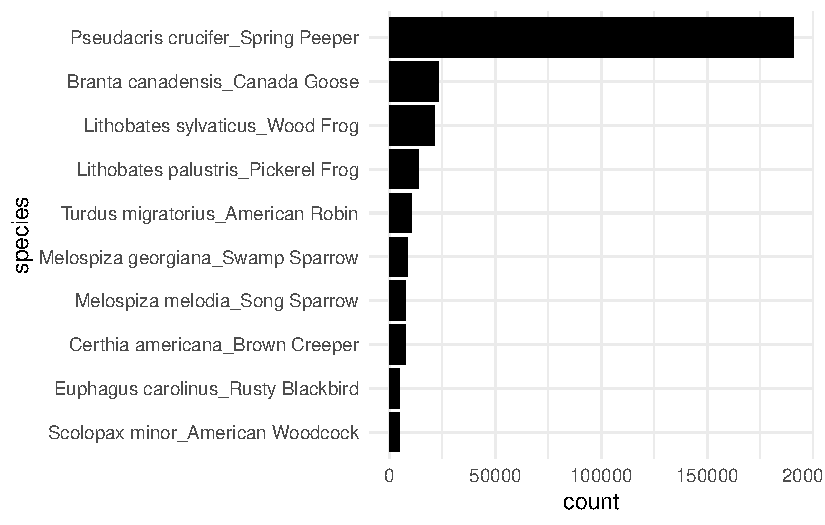
\includegraphics[keepaspectratio]{draft_paper_files/figure-pdf/unnamed-chunk-4-1.pdf}}

\linespread{2}

\linespread{0.9}

\begin{Shaded}
\begin{Highlighting}[]
\CommentTok{\# table 2:}
\NormalTok{site\_stats }\SpecialCharTok{|\textgreater{}} \FunctionTok{pander}\NormalTok{()}
\end{Highlighting}
\end{Shaded}

{\def\LTcaptype{none} % do not increment counter
\begin{longtable}[]{@{}
  >{\centering\arraybackslash}p{(\linewidth - 4\tabcolsep) * \real{0.2361}}
  >{\centering\arraybackslash}p{(\linewidth - 4\tabcolsep) * \real{0.1111}}
  >{\centering\arraybackslash}p{(\linewidth - 4\tabcolsep) * \real{0.2639}}@{}}
\toprule\noalign{}
\begin{minipage}[b]{\linewidth}\centering
deployment\_num
\end{minipage} & \begin{minipage}[b]{\linewidth}\centering
count
\end{minipage} & \begin{minipage}[b]{\linewidth}\centering
species\_richness
\end{minipage} \\
\midrule\noalign{}
\endhead
\bottomrule\noalign{}
\endlastfoot
AM0009 & 41192 & 8 \\
AM0007 & 34113 & 21 \\
AM0011 & 31651 & 7 \\
AM0001 & 30779 & 9 \\
AM0006 & 27854 & 22 \\
AM0018 & 23808 & 26 \\
AM0003 & 20493 & 17 \\
AM0014 & 20240 & 25 \\
AM0002 & 18238 & 18 \\
AM0015 & 11989 & 19 \\
\end{longtable}
}

\linespread{2}

To frame our analysis, we started investigating which temporal scale is
useful in comparing the eclipse to the surrounding days. We manipulated
the data to look at intervals around the time of totality (15:25:30) for
each day sampled to see what resolution best represented the differences
in species identifications during the eclipse. Fig 2 shows much more new
hits on the eclipse day compared to other days during intervals
extending to around 30 mins on either side of the time of totality. At
intervals of more than ± 30 mins, the number of identifications looks
similar to the other days.

\linespread{0.9}

\begin{Shaded}
\begin{Highlighting}[]
\NormalTok{days }\OtherTok{\textless{}{-}} \FunctionTok{c}\NormalTok{(}\DecValTok{1}\SpecialCharTok{:}\DecValTok{15}\NormalTok{)}

\DocumentationTok{\#\# units are all in seconds since midnight}

\DocumentationTok{\#\# create a vector of seconds that I want to add and subtract to and from}
\DocumentationTok{\#\# the time of totality}
\NormalTok{interval\_range }\OtherTok{\textless{}{-}}\NormalTok{ (}\FunctionTok{c}\NormalTok{(}\FunctionTok{seq}\NormalTok{(}\DecValTok{30}\NormalTok{, }\DecValTok{3030}\NormalTok{, }\AttributeTok{by =} \DecValTok{60}\NormalTok{)))}
\NormalTok{mid\_point }\OtherTok{\textless{}{-}} \FunctionTok{as\_hms}\NormalTok{(}\StringTok{"15:25:30"}\NormalTok{) }\SpecialCharTok{|\textgreater{}} \FunctionTok{as.numeric}\NormalTok{() }\DocumentationTok{\#\# time of totality}

\DocumentationTok{\#\# convert time to seconds since midnight}
\NormalTok{merged\_df }\OtherTok{\textless{}{-}}\NormalTok{ merged\_df }\SpecialCharTok{|\textgreater{}} \FunctionTok{mutate}\NormalTok{(}\AttributeTok{time\_basic =} \FunctionTok{as\_hms}\NormalTok{(time) }\SpecialCharTok{|\textgreater{}} \FunctionTok{as.numeric}\NormalTok{()) }\SpecialCharTok{|\textgreater{}}
  \FunctionTok{relocate}\NormalTok{(time\_basic)}
\DocumentationTok{\#\# only look at April 1 through 15}
\NormalTok{focused\_time }\OtherTok{\textless{}{-}}\NormalTok{ merged\_df }\SpecialCharTok{|\textgreater{}} \FunctionTok{filter}\NormalTok{(}\FunctionTok{day}\NormalTok{(date\_time) }\SpecialCharTok{\%in\%}\NormalTok{ days)}
\end{Highlighting}
\end{Shaded}

\linespread{2}

\linespread{0.9}

\begin{Shaded}
\begin{Highlighting}[]
\DocumentationTok{\#\# filter hits (of any species) based on a provided "interval" value}
\DocumentationTok{\#\# interval could be named better: it is really just the number of seconds}
\DocumentationTok{\#\# we are adding and subtracting from the time of totality}
\DocumentationTok{\#\# to create an interval}
\NormalTok{filter\_interval }\OtherTok{\textless{}{-}} \ControlFlowTok{function}\NormalTok{(mid\_point, df, interval, min\_prob) \{}
\NormalTok{  df }\SpecialCharTok{|\textgreater{}} \FunctionTok{filter}\NormalTok{(time\_basic }\SpecialCharTok{\textgreater{}=}\NormalTok{ mid\_point }\SpecialCharTok{{-}}\NormalTok{ interval }\SpecialCharTok{\&}\NormalTok{ time\_basic }\SpecialCharTok{\textless{}=}\NormalTok{ mid\_point }\SpecialCharTok{+}\NormalTok{ interval) }\SpecialCharTok{|\textgreater{}}
    \FunctionTok{mutate}\NormalTok{(}\AttributeTok{interval\_size =}\NormalTok{ interval }\SpecialCharTok{*} \DecValTok{2}\NormalTok{) }\SpecialCharTok{|\textgreater{}}
    \FunctionTok{filter}\NormalTok{(probability }\SpecialCharTok{\textgreater{}=}\NormalTok{ min\_prob)}
\NormalTok{\}}

\DocumentationTok{\#\# map through the function to get one data set filtered by each of the values in}
\DocumentationTok{\#\# the interval\_range variable}

\DocumentationTok{\#\# goal: see how the number of hits changes as we get a wider and wider interval around the eclipse}
\DocumentationTok{\#\# map through the function for the different interval sizes}
\NormalTok{dfs }\OtherTok{\textless{}{-}} \FunctionTok{map\_dfr}\NormalTok{(interval\_range, filter\_interval,}
               \AttributeTok{mid\_point =} \FunctionTok{as\_hms}\NormalTok{(}\StringTok{"15:25:30"}\NormalTok{) }\SpecialCharTok{|\textgreater{}} \FunctionTok{as.numeric}\NormalTok{(),}
               \AttributeTok{df =}\NormalTok{ focused\_time, }\AttributeTok{min\_prob =} \FloatTok{0.75}\NormalTok{) }\SpecialCharTok{|\textgreater{}}
                   \FunctionTok{mutate}\NormalTok{(}\AttributeTok{day =} \FunctionTok{day}\NormalTok{(date\_time),}
                          \AttributeTok{month =} \FunctionTok{month}\NormalTok{(date\_time),}
                          \AttributeTok{eclipse\_ind =} \FunctionTok{if\_else}\NormalTok{(day }\SpecialCharTok{==} \StringTok{"8"} \SpecialCharTok{\&}\NormalTok{ month }\SpecialCharTok{==} \StringTok{"4"}\NormalTok{,}
                                                \AttributeTok{true =} \StringTok{"eclipse"}\NormalTok{,}
                                        \AttributeTok{false =} \StringTok{"non{-}eclipse"}\NormalTok{))}
\end{Highlighting}
\end{Shaded}

\begin{verbatim}
New names:
New names:
New names:
New names:
New names:
New names:
New names:
New names:
New names:
New names:
New names:
New names:
New names:
New names:
New names:
New names:
New names:
New names:
New names:
New names:
New names:
New names:
New names:
New names:
New names:
New names:
New names:
New names:
New names:
New names:
New names:
New names:
New names:
New names:
New names:
New names:
New names:
New names:
New names:
New names:
New names:
New names:
New names:
New names:
New names:
New names:
New names:
New names:
New names:
New names:
New names:
* `...17` -> `...18`
\end{verbatim}

\begin{Shaded}
\begin{Highlighting}[]
\DocumentationTok{\#\# grab total number of detections (of any species) for each interval for}
\DocumentationTok{\#\# each day for each month (only looking at April here, but wanted}
\DocumentationTok{\#\# this to generalize to March if we included it).}
\NormalTok{df\_count }\OtherTok{\textless{}{-}}\NormalTok{ dfs }\SpecialCharTok{|\textgreater{}} \FunctionTok{group\_by}\NormalTok{(day, month, interval\_size) }\SpecialCharTok{|\textgreater{}}
  \FunctionTok{summarise}\NormalTok{(}\AttributeTok{n\_hits =} \FunctionTok{n}\NormalTok{(),}
    \AttributeTok{eclipse\_ind =} \FunctionTok{first}\NormalTok{(eclipse\_ind))}
\end{Highlighting}
\end{Shaded}

\begin{verbatim}
`summarise()` has grouped output by 'day', 'month'. You can override using the
`.groups` argument.
\end{verbatim}

\begin{Shaded}
\begin{Highlighting}[]
\DocumentationTok{\#\# n\_hits is cumulative for larger and larger interval sizes}
\DocumentationTok{\#\# new\_hits is the number of unique hits for each increasing interval }
\DocumentationTok{\#\# e.g., if there were 50 hits in the minute surrounding the eclipse and }
\DocumentationTok{\#\# 150 hits in the two minutes surrounding the eclipse, then}
\DocumentationTok{\#\# n\_hits would be (50, 200) and new\_hits would be (50, 150)}
\NormalTok{df\_count }\OtherTok{\textless{}{-}}\NormalTok{ df\_count }\SpecialCharTok{|\textgreater{}} \FunctionTok{group\_by}\NormalTok{(day, month) }\SpecialCharTok{|\textgreater{}}
  \FunctionTok{mutate}\NormalTok{(}\AttributeTok{n\_hits\_lag =} \FunctionTok{lag}\NormalTok{(n\_hits),}
         \AttributeTok{n\_hits\_lag =} \FunctionTok{if\_else}\NormalTok{(}\FunctionTok{is.na}\NormalTok{(n\_hits\_lag), }\AttributeTok{true =} \DecValTok{0}\NormalTok{, }\AttributeTok{false =}\NormalTok{ n\_hits\_lag)) }\SpecialCharTok{|\textgreater{}}
  \FunctionTok{mutate}\NormalTok{(}\AttributeTok{new\_hits =}\NormalTok{ n\_hits }\SpecialCharTok{{-}}\NormalTok{ n\_hits\_lag)}

\DocumentationTok{\#\# this second one is just the raw number of new hits as the interval size}
\DocumentationTok{\#\# surrounding the eclipse slowly increases by 1 minute on each side,}
\DocumentationTok{\#\# centered at totality}

\DocumentationTok{\#\# this suggests that there is an increase in overall call rate}
\DocumentationTok{\#\# during the eclipse but that we are looking too far out}
\DocumentationTok{\#\# the increasing amount of calls peters off as we get further from }
\DocumentationTok{\#\# totality and is no different than other days past}
\DocumentationTok{\#\# an interval size of about 2000 seconds (which roughly }
\DocumentationTok{\#\# corresponds to adding and subtracting 30 minutes from the time of totality)}
\FunctionTok{ggplot}\NormalTok{(}\AttributeTok{data =}\NormalTok{ df\_count, }\FunctionTok{aes}\NormalTok{(}\AttributeTok{x =}\NormalTok{ interval\_size, }\AttributeTok{y =}\NormalTok{ new\_hits)) }\SpecialCharTok{+}
  \FunctionTok{geom\_line}\NormalTok{(}\FunctionTok{aes}\NormalTok{(}\AttributeTok{group =}\NormalTok{ day, }\AttributeTok{colour =}\NormalTok{ eclipse\_ind), }\AttributeTok{alpha =} \FloatTok{0.5}\NormalTok{) }\SpecialCharTok{+}
  \FunctionTok{scale\_colour\_viridis\_d}\NormalTok{() }\SpecialCharTok{+}
  \FunctionTok{labs}\NormalTok{(}\AttributeTok{x =} \StringTok{"Interval Around Totality (seconds)"}\NormalTok{,}
  \AttributeTok{y =} \StringTok{"New Species Detections"}\NormalTok{,}
  \AttributeTok{colour =} \StringTok{"Day"}\NormalTok{)}\SpecialCharTok{+}
  \FunctionTok{theme\_minimal}\NormalTok{()}
\end{Highlighting}
\end{Shaded}

\pandocbounded{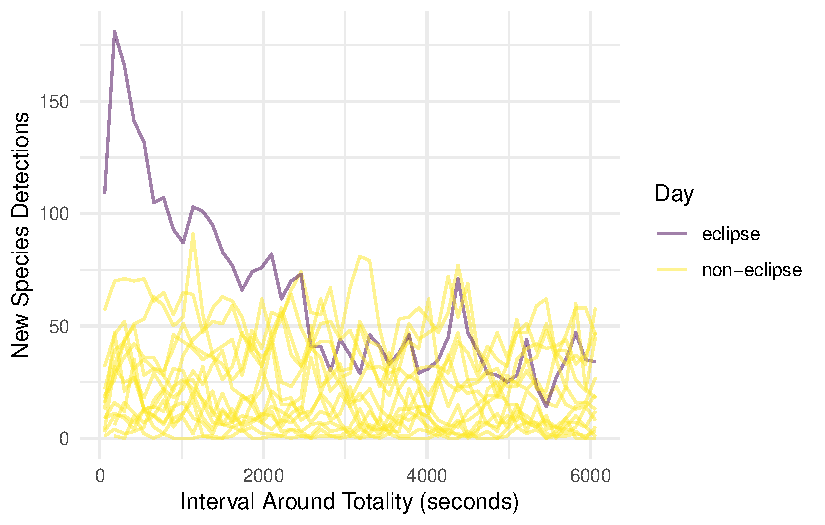
\includegraphics[keepaspectratio]{draft_paper_files/figure-pdf/unnamed-chunk-7-1.pdf}}

\linespread{2}

After finding our interval of interest, we moved into looking at the
vocalization pattern from all species on eclipse day compared to other
days. Fig 3 depects the presence of any species from all sites (1 for a
species identification and 0 for no species identified) during a span of
5 days including the date of the eclipse. During the day of the eclipse
(April 8th), there is a clear peak in activity centered right at the
time of totality, which is not present in other days.

\linespread{0.9}

\begin{Shaded}
\begin{Highlighting}[]
\CommentTok{\# 5 day span}
\NormalTok{day1 }\OtherTok{\textless{}{-}} \FunctionTok{ymd\_hms}\NormalTok{(}\StringTok{"2024{-}04{-}06 00:00:00"}\NormalTok{)}
\NormalTok{day5 }\OtherTok{\textless{}{-}} \FunctionTok{ymd\_hms}\NormalTok{(}\StringTok{"2024{-}04{-}10 23:59:59"}\NormalTok{)}

\CommentTok{\# eclipse time: 15:25:30}
\NormalTok{time\_start }\OtherTok{\textless{}{-}} \FunctionTok{as\_hms}\NormalTok{(}\StringTok{"14:55:30"}\NormalTok{)}
\NormalTok{time\_end }\OtherTok{\textless{}{-}} \FunctionTok{as\_hms}\NormalTok{(}\StringTok{"15:55:30"}\NormalTok{)}

\NormalTok{five\_day }\OtherTok{\textless{}{-}}\NormalTok{ merged\_df }\SpecialCharTok{|\textgreater{}} \FunctionTok{filter}\NormalTok{(}\FunctionTok{between}\NormalTok{(time, }
\NormalTok{time\_start, time\_end)) }\SpecialCharTok{|\textgreater{}}
  \FunctionTok{filter}\NormalTok{(day1 }\SpecialCharTok{\textless{}=}\NormalTok{ date\_time }\SpecialCharTok{\&}\NormalTok{ date\_time }\SpecialCharTok{\textless{}=}\NormalTok{ day5) }\SpecialCharTok{|\textgreater{}}
  \FunctionTok{mutate}\NormalTok{(}\AttributeTok{date =} \FunctionTok{as\_date}\NormalTok{(date\_time)) }\SpecialCharTok{|\textgreater{}} 
  \FunctionTok{group\_by}\NormalTok{(date, id) }\SpecialCharTok{|\textgreater{}} \CommentTok{\# want to complete the gaps for each site/AM}
  \FunctionTok{complete}\NormalTok{(}\AttributeTok{time =} \FunctionTok{as\_hms}\NormalTok{(}\FunctionTok{seq}\NormalTok{(}\FunctionTok{as.numeric}\NormalTok{(time\_start), }\FunctionTok{as.numeric}\NormalTok{(time\_end), }\AttributeTok{by =} \DecValTok{3}\NormalTok{)), }
  \AttributeTok{fill =} \FunctionTok{list}\NormalTok{(}\AttributeTok{value =} \ConstantTok{NA}\NormalTok{)) }\SpecialCharTok{|\textgreater{}} 
    \FunctionTok{ungroup}\NormalTok{() }\SpecialCharTok{|\textgreater{}} 
    \FunctionTok{mutate}\NormalTok{(}\AttributeTok{Presence =} \FunctionTok{if\_else}\NormalTok{(}\SpecialCharTok{!}\FunctionTok{is.na}\NormalTok{(probability),}
    \AttributeTok{true =} \DecValTok{1}\NormalTok{,}
    \AttributeTok{false =} \DecValTok{0}\NormalTok{)) }\SpecialCharTok{|\textgreater{}} 
      \FunctionTok{relocate}\NormalTok{(Presence, probability) }\SpecialCharTok{|\textgreater{}} 
      \FunctionTok{filter}\NormalTok{(}\FunctionTok{seconds}\NormalTok{(time) }\SpecialCharTok{!=} \DecValTok{57}\NormalTok{)}

\CommentTok{\# whole data set}
\FunctionTok{ggplot}\NormalTok{(five\_day, }\FunctionTok{aes}\NormalTok{(time, Presence))}\SpecialCharTok{+}
  \FunctionTok{geom\_jitter}\NormalTok{(}\AttributeTok{width =} \DecValTok{0}\NormalTok{, }\AttributeTok{height =} \FloatTok{0.05}\NormalTok{)}\SpecialCharTok{+}
  \FunctionTok{geom\_smooth}\NormalTok{(}\AttributeTok{se =}\NormalTok{ F)}\SpecialCharTok{+}
  \FunctionTok{facet\_wrap}\NormalTok{(}\SpecialCharTok{\textasciitilde{}}\FunctionTok{day}\NormalTok{(date))}\SpecialCharTok{+}
  \FunctionTok{scale\_x\_time}\NormalTok{()}\SpecialCharTok{+}
  \FunctionTok{theme\_minimal}\NormalTok{()}
\end{Highlighting}
\end{Shaded}

\begin{verbatim}
`geom_smooth()` using method = 'gam' and formula = 'y ~ s(x, bs = "cs")'
\end{verbatim}

\pandocbounded{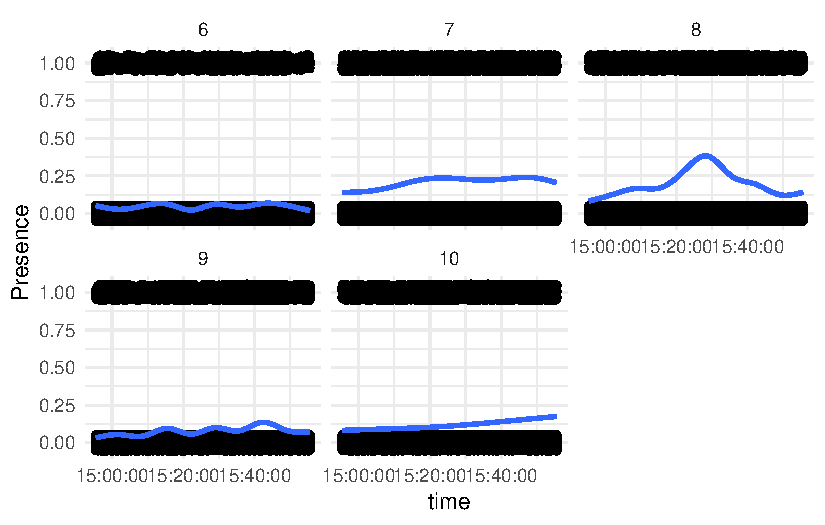
\includegraphics[keepaspectratio]{draft_paper_files/figure-pdf/unnamed-chunk-8-1.pdf}}

\linespread{2}

Then, we looked at the most common species for this 5 day span during
the time span of ±30 from the time of the eclipse (Table 1).

\linespread{0.9}

\begin{Shaded}
\begin{Highlighting}[]
\NormalTok{top\_ten\_5d }\OtherTok{\textless{}{-}}\NormalTok{ five\_day }\SpecialCharTok{|\textgreater{}} \FunctionTok{filter}\NormalTok{(}\SpecialCharTok{!}\FunctionTok{is.na}\NormalTok{(probability)) }\SpecialCharTok{|\textgreater{}} 
  \FunctionTok{group\_by}\NormalTok{(species) }\SpecialCharTok{|\textgreater{}} 
  \FunctionTok{summarise}\NormalTok{(}\AttributeTok{count =} \FunctionTok{n}\NormalTok{()) }\SpecialCharTok{|\textgreater{}} 
  \FunctionTok{arrange}\NormalTok{(}\FunctionTok{desc}\NormalTok{(count)) }\SpecialCharTok{|\textgreater{}} 
  \FunctionTok{slice}\NormalTok{(}\DecValTok{1}\SpecialCharTok{:}\DecValTok{10}\NormalTok{)}

\NormalTok{top\_ten\_5d }\SpecialCharTok{|\textgreater{}} \FunctionTok{pander}\NormalTok{()}
\end{Highlighting}
\end{Shaded}

{\def\LTcaptype{none} % do not increment counter
\begin{longtable}[]{@{}
  >{\centering\arraybackslash}p{(\linewidth - 2\tabcolsep) * \real{0.4583}}
  >{\centering\arraybackslash}p{(\linewidth - 2\tabcolsep) * \real{0.1111}}@{}}
\toprule\noalign{}
\begin{minipage}[b]{\linewidth}\centering
species
\end{minipage} & \begin{minipage}[b]{\linewidth}\centering
count
\end{minipage} \\
\midrule\noalign{}
\endhead
\bottomrule\noalign{}
\endlastfoot
Pseudacris crucifer\_Spring Peeper & 7931 \\
Lithobates sylvaticus\_Wood Frog & 2574 \\
Branta canadensis\_Canada Goose & 764 \\
Lithobates palustris\_Pickerel Frog & 709 \\
Poecile atricapillus\_Black-capped Chickadee & 582 \\
Quiscalus quiscula\_Common Grackle & 476 \\
Certhia americana\_Brown Creeper & 317 \\
Corvus brachyrhynchos\_American Crow & 295 \\
Meleagris gallopavo\_Wild Turkey & 286 \\
Sayornis phoebe\_Eastern Phoebe & 226 \\
\end{longtable}
}

\linespread{2}

\emph{Note: these contain those erroneous species}

(of those that are native) Next, we investigated the vocalization
activity for the most common species at the time of the eclipse across
the five days. First with Spring Peepers, the most common species in the
entire data set, we see similar peak in activity around the time of
totality (Fig 4). What is notable about April 6th was the low
temperature (fill in), which could have influence their activity.

\linespread{0.9}

\begin{Shaded}
\begin{Highlighting}[]
\NormalTok{sp\_5d }\OtherTok{\textless{}{-}}\NormalTok{ five\_day }\SpecialCharTok{|\textgreater{}} \FunctionTok{filter}\NormalTok{(species }\SpecialCharTok{==} \StringTok{"Pseudacris crucifer\_Spring Peeper"}\NormalTok{) }\SpecialCharTok{|\textgreater{}}
  \FunctionTok{group\_by}\NormalTok{(date, id) }\SpecialCharTok{|\textgreater{}} 
  \FunctionTok{complete}\NormalTok{(}\AttributeTok{time =} \FunctionTok{as\_hms}\NormalTok{(}\FunctionTok{seq}\NormalTok{(}\FunctionTok{as.numeric}\NormalTok{(time\_start), }\FunctionTok{as.numeric}\NormalTok{(time\_end), }\AttributeTok{by =} \DecValTok{3}\NormalTok{)), }
  \AttributeTok{fill =} \FunctionTok{list}\NormalTok{(}\AttributeTok{value =} \ConstantTok{NA}\NormalTok{)) }\SpecialCharTok{|\textgreater{}}
  \FunctionTok{mutate}\NormalTok{(}\AttributeTok{Presence =} \FunctionTok{if\_else}\NormalTok{(}\SpecialCharTok{!}\FunctionTok{is.na}\NormalTok{(probability),}
    \AttributeTok{true =} \DecValTok{1}\NormalTok{,}
    \AttributeTok{false =} \DecValTok{0}\NormalTok{)) }\SpecialCharTok{|\textgreater{}} 
  \FunctionTok{filter}\NormalTok{(}\FunctionTok{seconds}\NormalTok{(time) }\SpecialCharTok{!=} \DecValTok{57}\NormalTok{)}

\FunctionTok{ggplot}\NormalTok{(sp\_5d, }\FunctionTok{aes}\NormalTok{(time, Presence))}\SpecialCharTok{+}
  \FunctionTok{geom\_jitter}\NormalTok{(}\AttributeTok{width =} \DecValTok{0}\NormalTok{, }\AttributeTok{height =} \FloatTok{0.05}\NormalTok{)}\SpecialCharTok{+}
  \FunctionTok{geom\_smooth}\NormalTok{(}\AttributeTok{se =}\NormalTok{ F)}\SpecialCharTok{+}
  \FunctionTok{facet\_wrap}\NormalTok{(}\SpecialCharTok{\textasciitilde{}}\FunctionTok{day}\NormalTok{(date))}\SpecialCharTok{+}
  \FunctionTok{scale\_x\_time}\NormalTok{()}\SpecialCharTok{+}
  \FunctionTok{theme\_minimal}\NormalTok{()}
\end{Highlighting}
\end{Shaded}

\begin{verbatim}
`geom_smooth()` using method = 'gam' and formula = 'y ~ s(x, bs = "cs")'
\end{verbatim}

\pandocbounded{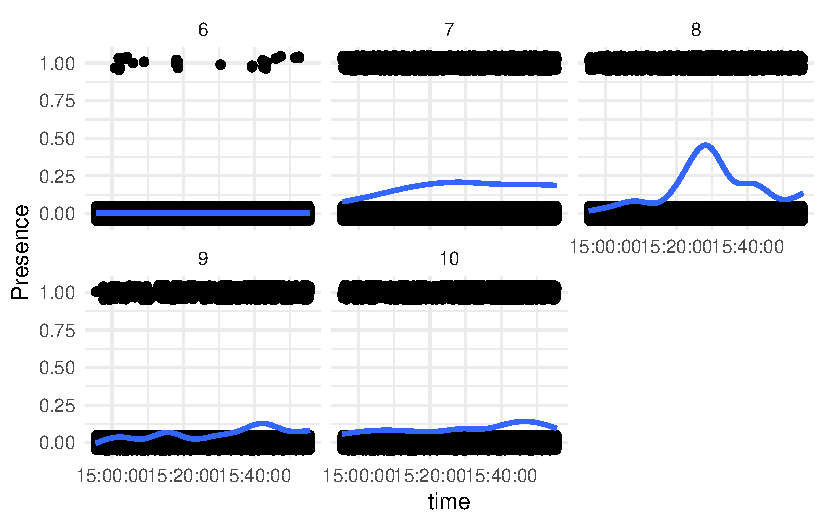
\includegraphics[keepaspectratio]{draft_paper_files/figure-pdf/unnamed-chunk-10-1.pdf}}

\linespread{2}

The wood frog was next most common for this time scale, and it a more
random pattern across the five days (Fig 5). It was not recorded at all
on April 6th (we again hypothesize the weather being an influence), and
the eclipse day does not seem to have a distinct pattern.

\linespread{0.9}

\begin{Shaded}
\begin{Highlighting}[]
\NormalTok{wf\_5d }\OtherTok{\textless{}{-}}\NormalTok{ five\_day }\SpecialCharTok{|\textgreater{}} \FunctionTok{filter}\NormalTok{(species }\SpecialCharTok{==} \StringTok{"Lithobates sylvaticus\_Wood Frog"}\NormalTok{) }\SpecialCharTok{|\textgreater{}}
  \FunctionTok{group\_by}\NormalTok{(date, id) }\SpecialCharTok{|\textgreater{}} 
  \FunctionTok{complete}\NormalTok{(}\AttributeTok{time =} \FunctionTok{as\_hms}\NormalTok{(}\FunctionTok{seq}\NormalTok{(}\FunctionTok{as.numeric}\NormalTok{(time\_start), }\FunctionTok{as.numeric}\NormalTok{(time\_end), }\AttributeTok{by =} \DecValTok{3}\NormalTok{)), }
  \AttributeTok{fill =} \FunctionTok{list}\NormalTok{(}\AttributeTok{value =} \ConstantTok{NA}\NormalTok{)) }\SpecialCharTok{|\textgreater{}}
  \FunctionTok{mutate}\NormalTok{(}\AttributeTok{Presence =} \FunctionTok{if\_else}\NormalTok{(}\SpecialCharTok{!}\FunctionTok{is.na}\NormalTok{(probability),}
    \AttributeTok{true =} \DecValTok{1}\NormalTok{,}
    \AttributeTok{false =} \DecValTok{0}\NormalTok{)) }\SpecialCharTok{|\textgreater{}} 
  \FunctionTok{filter}\NormalTok{(}\FunctionTok{seconds}\NormalTok{(time) }\SpecialCharTok{!=} \DecValTok{57}\NormalTok{)}

\FunctionTok{ggplot}\NormalTok{(wf\_5d, }\FunctionTok{aes}\NormalTok{(time, Presence))}\SpecialCharTok{+}
  \FunctionTok{geom\_jitter}\NormalTok{(}\AttributeTok{width =} \DecValTok{0}\NormalTok{, }\AttributeTok{height =} \FloatTok{0.05}\NormalTok{)}\SpecialCharTok{+}
  \FunctionTok{geom\_smooth}\NormalTok{(}\AttributeTok{se =}\NormalTok{ F)}\SpecialCharTok{+}
  \FunctionTok{facet\_wrap}\NormalTok{(}\SpecialCharTok{\textasciitilde{}}\FunctionTok{day}\NormalTok{(date))}\SpecialCharTok{+}
  \FunctionTok{scale\_x\_time}\NormalTok{()}\SpecialCharTok{+}
  \FunctionTok{theme\_minimal}\NormalTok{()}
\end{Highlighting}
\end{Shaded}

\begin{verbatim}
`geom_smooth()` using method = 'gam' and formula = 'y ~ s(x, bs = "cs")'
\end{verbatim}

\pandocbounded{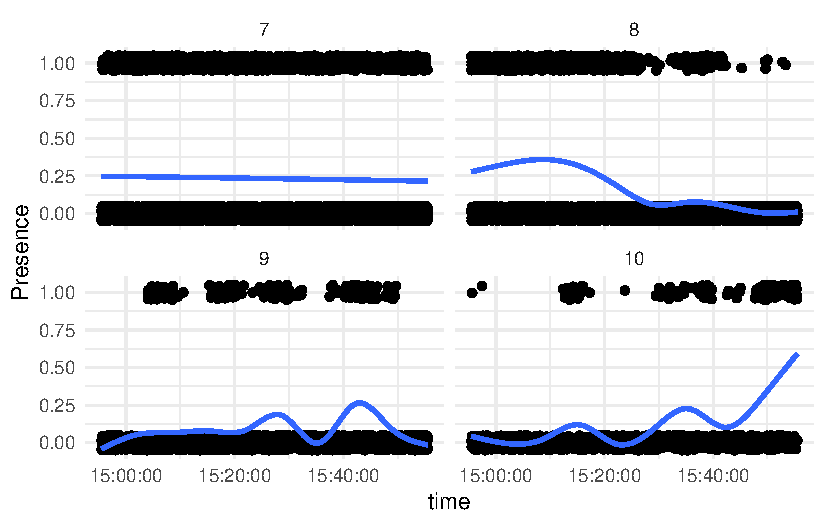
\includegraphics[keepaspectratio]{draft_paper_files/figure-pdf/unnamed-chunk-11-1.pdf}}

\linespread{2}

The Canada goose was the most common bird species across the 5 days for
this time scale (Table 1). It's overall pattern across the 5 days does
not seem different, but there's a notable gap in presence directly at
the time of totality (Fig 6).

\linespread{0.9}

\begin{Shaded}
\begin{Highlighting}[]
\NormalTok{cgo\_5d }\OtherTok{\textless{}{-}}\NormalTok{ five\_day }\SpecialCharTok{|\textgreater{}} \FunctionTok{filter}\NormalTok{(species }\SpecialCharTok{==} \StringTok{"Branta canadensis\_Canada Goose"}\NormalTok{) }\SpecialCharTok{|\textgreater{}}
  \FunctionTok{group\_by}\NormalTok{(date, id) }\SpecialCharTok{|\textgreater{}} 
  \FunctionTok{complete}\NormalTok{(}\AttributeTok{time =} \FunctionTok{as\_hms}\NormalTok{(}\FunctionTok{seq}\NormalTok{(}\FunctionTok{as.numeric}\NormalTok{(time\_start), }\FunctionTok{as.numeric}\NormalTok{(time\_end), }\AttributeTok{by =} \DecValTok{3}\NormalTok{)), }
  \AttributeTok{fill =} \FunctionTok{list}\NormalTok{(}\AttributeTok{value =} \ConstantTok{NA}\NormalTok{)) }\SpecialCharTok{|\textgreater{}}
  \FunctionTok{mutate}\NormalTok{(}\AttributeTok{Presence =} \FunctionTok{if\_else}\NormalTok{(}\SpecialCharTok{!}\FunctionTok{is.na}\NormalTok{(probability),}
    \AttributeTok{true =} \DecValTok{1}\NormalTok{,}
    \AttributeTok{false =} \DecValTok{0}\NormalTok{)) }\SpecialCharTok{|\textgreater{}} 
  \FunctionTok{filter}\NormalTok{(}\FunctionTok{seconds}\NormalTok{(time) }\SpecialCharTok{!=} \DecValTok{57}\NormalTok{)}

\FunctionTok{ggplot}\NormalTok{(cgo\_5d, }\FunctionTok{aes}\NormalTok{(time, Presence))}\SpecialCharTok{+}
  \FunctionTok{geom\_jitter}\NormalTok{(}\AttributeTok{width =} \DecValTok{0}\NormalTok{, }\AttributeTok{height =} \FloatTok{0.05}\NormalTok{)}\SpecialCharTok{+}
  \FunctionTok{geom\_smooth}\NormalTok{(}\AttributeTok{se =}\NormalTok{ F)}\SpecialCharTok{+}
  \FunctionTok{facet\_wrap}\NormalTok{(}\SpecialCharTok{\textasciitilde{}}\FunctionTok{day}\NormalTok{(date))}\SpecialCharTok{+}
  \FunctionTok{scale\_x\_time}\NormalTok{()}\SpecialCharTok{+}
  \FunctionTok{theme\_minimal}\NormalTok{()}
\end{Highlighting}
\end{Shaded}

\begin{verbatim}
`geom_smooth()` using method = 'gam' and formula = 'y ~ s(x, bs = "cs")'
\end{verbatim}

\pandocbounded{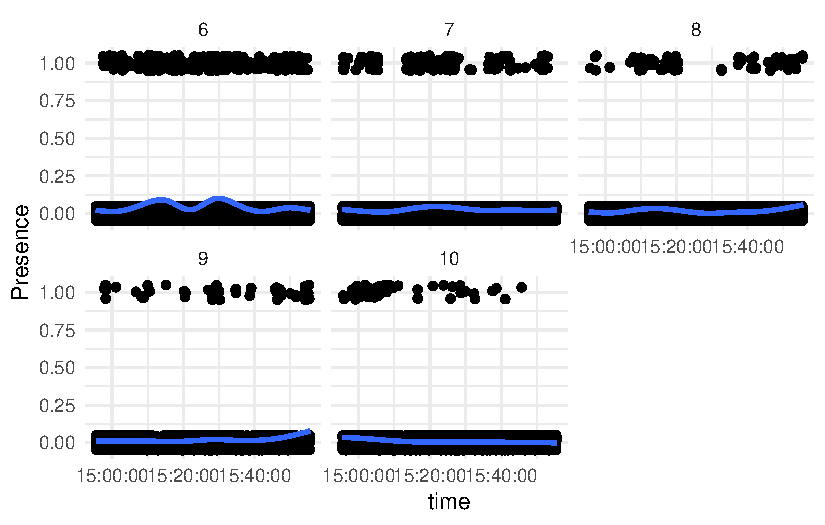
\includegraphics[keepaspectratio]{draft_paper_files/figure-pdf/unnamed-chunk-12-1.pdf}}

\linespread{2}

The last frog in the top ten, the pickerel frog, had a similar pattern
to the Spring Peeper, but a lot less dramatic (Fig 7). Like the wood
frog, it was also not detected on the 6th. However, there is a slight
increase in detections around the time of totality, but it is very
minimal (Fig 7).

\linespread{0.9}

\begin{Shaded}
\begin{Highlighting}[]
\NormalTok{pf\_5d }\OtherTok{\textless{}{-}}\NormalTok{ five\_day }\SpecialCharTok{|\textgreater{}} \FunctionTok{filter}\NormalTok{(species }\SpecialCharTok{==} \StringTok{"Lithobates palustris\_Pickerel Frog"}\NormalTok{) }\SpecialCharTok{|\textgreater{}}
  \FunctionTok{group\_by}\NormalTok{(date, id) }\SpecialCharTok{|\textgreater{}} 
  \FunctionTok{complete}\NormalTok{(}\AttributeTok{time =} \FunctionTok{as\_hms}\NormalTok{(}\FunctionTok{seq}\NormalTok{(}\FunctionTok{as.numeric}\NormalTok{(time\_start), }\FunctionTok{as.numeric}\NormalTok{(time\_end), }\AttributeTok{by =} \DecValTok{3}\NormalTok{)), }
  \AttributeTok{fill =} \FunctionTok{list}\NormalTok{(}\AttributeTok{value =} \ConstantTok{NA}\NormalTok{)) }\SpecialCharTok{|\textgreater{}}
  \FunctionTok{mutate}\NormalTok{(}\AttributeTok{Presence =} \FunctionTok{if\_else}\NormalTok{(}\SpecialCharTok{!}\FunctionTok{is.na}\NormalTok{(probability),}
    \AttributeTok{true =} \DecValTok{1}\NormalTok{,}
    \AttributeTok{false =} \DecValTok{0}\NormalTok{)) }\SpecialCharTok{|\textgreater{}} 
  \FunctionTok{filter}\NormalTok{(}\FunctionTok{seconds}\NormalTok{(time) }\SpecialCharTok{!=} \DecValTok{57}\NormalTok{)}

\FunctionTok{ggplot}\NormalTok{(pf\_5d, }\FunctionTok{aes}\NormalTok{(time, Presence))}\SpecialCharTok{+}
  \FunctionTok{geom\_jitter}\NormalTok{(}\AttributeTok{width =} \DecValTok{0}\NormalTok{, }\AttributeTok{height =} \FloatTok{0.05}\NormalTok{)}\SpecialCharTok{+}
  \FunctionTok{geom\_smooth}\NormalTok{(}\AttributeTok{se =}\NormalTok{ F)}\SpecialCharTok{+}
  \FunctionTok{facet\_wrap}\NormalTok{(}\SpecialCharTok{\textasciitilde{}}\FunctionTok{day}\NormalTok{(date))}\SpecialCharTok{+}
  \FunctionTok{scale\_x\_time}\NormalTok{()}\SpecialCharTok{+}
  \FunctionTok{theme\_minimal}\NormalTok{()}
\end{Highlighting}
\end{Shaded}

\begin{verbatim}
`geom_smooth()` using method = 'gam' and formula = 'y ~ s(x, bs = "cs")'
\end{verbatim}

\pandocbounded{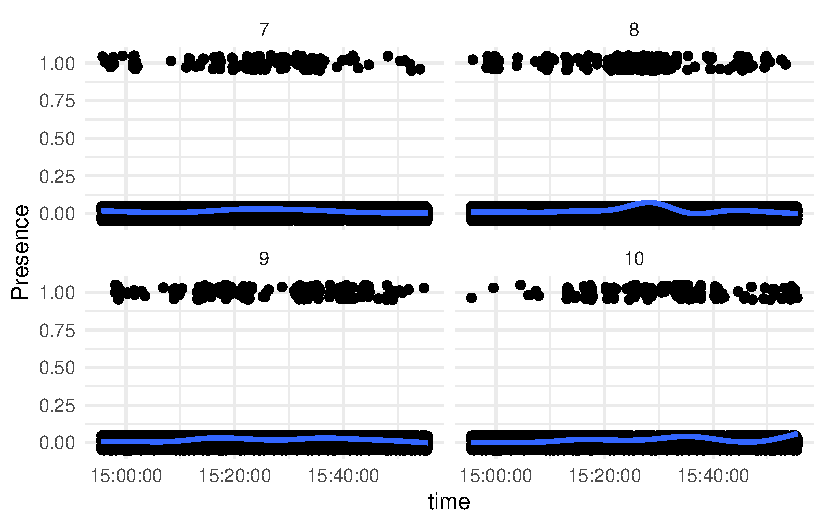
\includegraphics[keepaspectratio]{draft_paper_files/figure-pdf/unnamed-chunk-13-1.pdf}}

\linespread{2}

The next bird we looked at was the Black-capped Chickadee. There is much
of a discernible visual pattern, especially due to the lack of
detections on the 7th and 8th (Fig 8).

\linespread{0.9}

\begin{Shaded}
\begin{Highlighting}[]
\NormalTok{bcc\_5d }\OtherTok{\textless{}{-}}\NormalTok{ five\_day }\SpecialCharTok{|\textgreater{}} \FunctionTok{filter}\NormalTok{(species }\SpecialCharTok{==} \StringTok{"Poecile atricapillus\_Black{-}capped Chickadee"}\NormalTok{) }\SpecialCharTok{|\textgreater{}}
  \FunctionTok{group\_by}\NormalTok{(date, id) }\SpecialCharTok{|\textgreater{}} 
  \FunctionTok{complete}\NormalTok{(}\AttributeTok{time =} \FunctionTok{as\_hms}\NormalTok{(}\FunctionTok{seq}\NormalTok{(}\FunctionTok{as.numeric}\NormalTok{(time\_start), }\FunctionTok{as.numeric}\NormalTok{(time\_end), }\AttributeTok{by =} \DecValTok{3}\NormalTok{)), }
  \AttributeTok{fill =} \FunctionTok{list}\NormalTok{(}\AttributeTok{value =} \ConstantTok{NA}\NormalTok{)) }\SpecialCharTok{|\textgreater{}}
  \FunctionTok{mutate}\NormalTok{(}\AttributeTok{Presence =} \FunctionTok{if\_else}\NormalTok{(}\SpecialCharTok{!}\FunctionTok{is.na}\NormalTok{(probability),}
    \AttributeTok{true =} \DecValTok{1}\NormalTok{,}
    \AttributeTok{false =} \DecValTok{0}\NormalTok{)) }\SpecialCharTok{|\textgreater{}} 
  \FunctionTok{filter}\NormalTok{(}\FunctionTok{seconds}\NormalTok{(time) }\SpecialCharTok{!=} \DecValTok{57}\NormalTok{)}

\FunctionTok{ggplot}\NormalTok{(bcc\_5d, }\FunctionTok{aes}\NormalTok{(time, Presence))}\SpecialCharTok{+}
  \FunctionTok{geom\_jitter}\NormalTok{(}\AttributeTok{width =} \DecValTok{0}\NormalTok{, }\AttributeTok{height =} \FloatTok{0.05}\NormalTok{)}\SpecialCharTok{+}
  \FunctionTok{geom\_smooth}\NormalTok{(}\AttributeTok{se =}\NormalTok{ F)}\SpecialCharTok{+}
  \FunctionTok{facet\_wrap}\NormalTok{(}\SpecialCharTok{\textasciitilde{}}\FunctionTok{day}\NormalTok{(date))}\SpecialCharTok{+}
  \FunctionTok{scale\_x\_time}\NormalTok{()}\SpecialCharTok{+}
  \FunctionTok{theme\_minimal}\NormalTok{()}
\end{Highlighting}
\end{Shaded}

\begin{verbatim}
`geom_smooth()` using method = 'gam' and formula = 'y ~ s(x, bs = "cs")'
\end{verbatim}

\pandocbounded{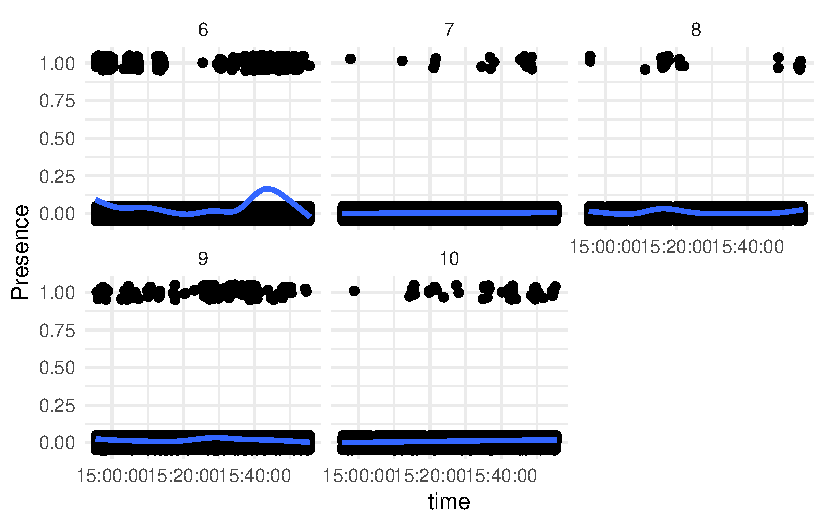
\includegraphics[keepaspectratio]{draft_paper_files/figure-pdf/unnamed-chunk-14-1.pdf}}

\linespread{2}

The Common Grackle seemed to have a more dramatic response to the
eclipse (Fig 9). Even more clearly than the Canadian Goose, there is a
gap in detection around the time of totality, but lots of detections
leading up to totality (during the partial eclipse). Partially what
makes this pattern so distinct is the high number of calls on the 7th
that did not match the pattern seen on the eclipse (Fig 9). However,
there were a lot more calls on the 7th and 8th than the other
surrounding days, which makes the comparison less robust.

\linespread{0.9}

\begin{Shaded}
\begin{Highlighting}[]
\NormalTok{cgr\_5d }\OtherTok{\textless{}{-}}\NormalTok{ five\_day }\SpecialCharTok{|\textgreater{}} \FunctionTok{filter}\NormalTok{(species }\SpecialCharTok{==} \StringTok{"Quiscalus quiscula\_Common Grackle"}\NormalTok{) }\SpecialCharTok{|\textgreater{}}
  \FunctionTok{group\_by}\NormalTok{(date, id) }\SpecialCharTok{|\textgreater{}} 
  \FunctionTok{complete}\NormalTok{(}\AttributeTok{time =} \FunctionTok{as\_hms}\NormalTok{(}\FunctionTok{seq}\NormalTok{(}\FunctionTok{as.numeric}\NormalTok{(time\_start), }\FunctionTok{as.numeric}\NormalTok{(time\_end), }\AttributeTok{by =} \DecValTok{3}\NormalTok{)), }
  \AttributeTok{fill =} \FunctionTok{list}\NormalTok{(}\AttributeTok{value =} \ConstantTok{NA}\NormalTok{)) }\SpecialCharTok{|\textgreater{}}
  \FunctionTok{mutate}\NormalTok{(}\AttributeTok{Presence =} \FunctionTok{if\_else}\NormalTok{(}\SpecialCharTok{!}\FunctionTok{is.na}\NormalTok{(probability),}
    \AttributeTok{true =} \DecValTok{1}\NormalTok{,}
    \AttributeTok{false =} \DecValTok{0}\NormalTok{)) }\SpecialCharTok{|\textgreater{}} 
  \FunctionTok{filter}\NormalTok{(}\FunctionTok{seconds}\NormalTok{(time) }\SpecialCharTok{!=} \DecValTok{57}\NormalTok{)}

\FunctionTok{ggplot}\NormalTok{(cgr\_5d, }\FunctionTok{aes}\NormalTok{(time, Presence))}\SpecialCharTok{+}
  \FunctionTok{geom\_jitter}\NormalTok{(}\AttributeTok{width =} \DecValTok{0}\NormalTok{, }\AttributeTok{height =} \FloatTok{0.05}\NormalTok{)}\SpecialCharTok{+}
  \FunctionTok{geom\_smooth}\NormalTok{(}\AttributeTok{se =}\NormalTok{ F)}\SpecialCharTok{+}
  \FunctionTok{facet\_wrap}\NormalTok{(}\SpecialCharTok{\textasciitilde{}}\FunctionTok{day}\NormalTok{(date))}\SpecialCharTok{+}
  \FunctionTok{scale\_x\_time}\NormalTok{()}\SpecialCharTok{+}
  \FunctionTok{theme\_minimal}\NormalTok{()}
\end{Highlighting}
\end{Shaded}

\begin{verbatim}
`geom_smooth()` using method = 'gam' and formula = 'y ~ s(x, bs = "cs")'
\end{verbatim}

\pandocbounded{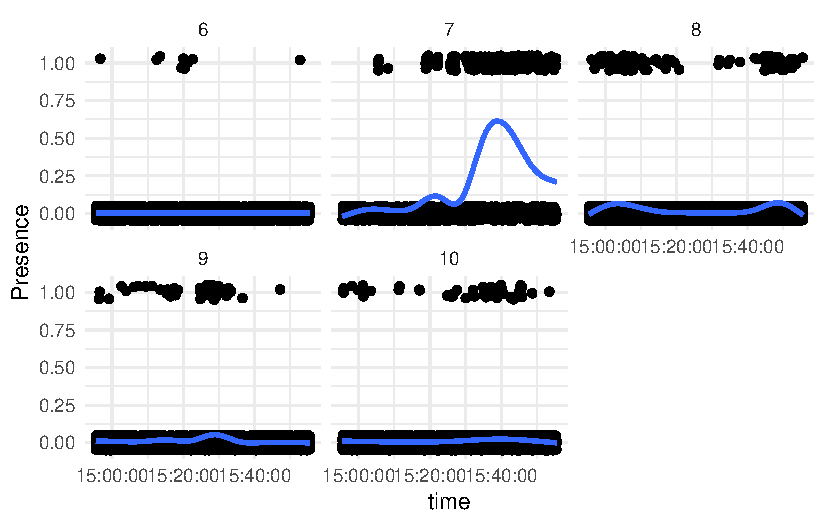
\includegraphics[keepaspectratio]{draft_paper_files/figure-pdf/unnamed-chunk-15-1.pdf}}

\linespread{2}

After looking at vizuals of species specific-responses and the entire
data set of detections there seems to be a difference in responses
between some of the frogs and birds. There also seems to be three
categories of responses in general: no response to the eclipse,
increased calls around totality, and a gap in calls at totality (but
perhaps increased calls during totality). These differences in responses
may reflect differences in light-triggered behaviors, which prompted us
to do more formal analysis and modeling.

\section{Community Model}\label{community-model}

\linespread{0.9}

\begin{Shaded}
\begin{Highlighting}[]
\NormalTok{com\_mod }\OtherTok{\textless{}{-}} \FunctionTok{readRDS}\NormalTok{(}\FunctionTok{here}\NormalTok{(}\StringTok{"Scripts/AM\_6\_3d\_mod.rds"}\NormalTok{))}
\end{Highlighting}
\end{Shaded}

\linespread{2}

To model all the species identified at \_\_ sites and over \_\_\_ days
(centered on the day of eclipse), we used a generalized additive mixed
model. The mixed model component incorporates a autoregressive term to
address autocorrelation in the data. We used species detection --
whether BirdNET identified a species or not -- as our binary response
variable. We wanted to see the overall community reaction to the eclipse
in this model, so all species were included in the analysis. Any
3-second time span where BirdNET predicted a species, we coded a 1 and
any other 3-second soundbyte was coded as a 0.

\[
\operatorname{logit}(\pi_{iad}) = \beta_{ad} + f_{ad}(t_{iad}) + \epsilon_{iad}
\]

Since the response variable is binary, our `family' for the model was
binomial and we used a log-link function. \(\pi_{id}\) represents the
probability of detecting a species for the \(i^{th}\) observation
recorded on the \(a^{th}\) audiomoth(\(a = 1, 2, \ldots, __\)) on the
\(d^{th}\) day of recording (\(d = _______\)). \(\beta_{ad}\) is the
intercept for each audiomoth-day combination. \(f_{ad}(t_{iad})\) is a
smoother term for time (indexed by \(i\)) that changes for each
audiomoth-day combination. \(t_{iad}\) represents the time (in seconds)
that the \(i^{th}\) observation was recorded at the \(a^{th}\) audiomoth
and the \(d^{th}\) day. \(\epsilon_{iad}\) represents random errors that
follow an AR(1) temporal correlation structure for each AudioMoth-day
combination with common shared correlation parameter \(p\).

We saw that the smoothers were generally significant, meaning they
effectively caputured the pattern of species vocalization activity at
each site (AudioMoth) and day combination.

\linespread{0.9}

\begin{Shaded}
\begin{Highlighting}[]
\FunctionTok{tidy}\NormalTok{(com\_mod}\SpecialCharTok{$}\NormalTok{gam) }\SpecialCharTok{|\textgreater{}} \FunctionTok{pander}\NormalTok{()}
\end{Highlighting}
\end{Shaded}

{\def\LTcaptype{none} % do not increment counter
\begin{longtable}[]{@{}
  >{\centering\arraybackslash}p{(\linewidth - 8\tabcolsep) * \real{0.4675}}
  >{\centering\arraybackslash}p{(\linewidth - 8\tabcolsep) * \real{0.1039}}
  >{\centering\arraybackslash}p{(\linewidth - 8\tabcolsep) * \real{0.1169}}
  >{\centering\arraybackslash}p{(\linewidth - 8\tabcolsep) * \real{0.1558}}
  >{\centering\arraybackslash}p{(\linewidth - 8\tabcolsep) * \real{0.1558}}@{}}
\toprule\noalign{}
\begin{minipage}[b]{\linewidth}\centering
term
\end{minipage} & \begin{minipage}[b]{\linewidth}\centering
edf
\end{minipage} & \begin{minipage}[b]{\linewidth}\centering
ref.df
\end{minipage} & \begin{minipage}[b]{\linewidth}\centering
statistic
\end{minipage} & \begin{minipage}[b]{\linewidth}\centering
p.value
\end{minipage} \\
\midrule\noalign{}
\endhead
\bottomrule\noalign{}
\endlastfoot
s(time\_num):audiomoth\_dayAM0001.7 & 6.868 & 6.868 & 12.91 & 0 \\
s(time\_num):audiomoth\_dayAM0002.7 & 6.71 & 6.71 & 4.903 & 2.806e-05 \\
s(time\_num):audiomoth\_dayAM0009.7 & 7.18 & 7.18 & 127.2 & 0 \\
s(time\_num):audiomoth\_dayAM0011.7 & 1.791 & 1.791 & 1.022 & 0.2888 \\
s(time\_num):audiomoth\_dayAM0017.7 & 1 & 1 & 57.74 & 0 \\
s(time\_num):audiomoth\_dayAM0020.7 & 1 & 1 & 2.767 & 0.09622 \\
s(time\_num):audiomoth\_dayAM0001.8 & 8.604 & 8.604 & 87.65 & 0 \\
s(time\_num):audiomoth\_dayAM0002.8 & 7.363 & 7.363 & 54 & 0 \\
s(time\_num):audiomoth\_dayAM0009.8 & 5.23 & 5.23 & 17.24 & 0 \\
s(time\_num):audiomoth\_dayAM0011.8 & 7.84 & 7.84 & 39.83 & 0 \\
s(time\_num):audiomoth\_dayAM0017.8 & 6.617 & 6.617 & 23.93 & 0 \\
s(time\_num):audiomoth\_dayAM0020.8 & 3.195 & 3.195 & 4.144 &
0.004662 \\
s(time\_num):audiomoth\_dayAM0001.9 & 1 & 1 & 34.45 & 0 \\
s(time\_num):audiomoth\_dayAM0002.9 & 1 & 1 & 0.3167 & 0.5736 \\
s(time\_num):audiomoth\_dayAM0009.9 & 1 & 1 & 194.9 & 0 \\
s(time\_num):audiomoth\_dayAM0011.9 & 8.448 & 8.448 & 15 & 0 \\
s(time\_num):audiomoth\_dayAM0017.9 & 3.16 & 3.16 & 11.29 & 1.738e-07 \\
s(time\_num):audiomoth\_dayAM0020.9 & 1 & 1 & 0.9676 & 0.3253 \\
\end{longtable}
}

\linespread{2}

As seen with the smoothers and in the plot below, the day and the site
seems to result in a different pattern. We do still see the increase in
overall vocalizations on April 8th, but the patterns become more varied
from a peak at totality due to the site.

\linespread{0.9}

\begin{Shaded}
\begin{Highlighting}[]
\CommentTok{\# 3 day span}
\NormalTok{day1 }\OtherTok{\textless{}{-}} \FunctionTok{ymd\_hms}\NormalTok{(}\StringTok{"2024{-}04{-}07 00:00:00"}\NormalTok{)}
\NormalTok{day3 }\OtherTok{\textless{}{-}} \FunctionTok{ymd\_hms}\NormalTok{(}\StringTok{"2024{-}04{-}9 23:59:59"}\NormalTok{)}

\CommentTok{\# eclipse time: 15:25:30}
\NormalTok{time\_start }\OtherTok{\textless{}{-}} \FunctionTok{as\_hms}\NormalTok{(}\StringTok{"14:55:30"}\NormalTok{)}
\NormalTok{time\_end }\OtherTok{\textless{}{-}} \FunctionTok{as\_hms}\NormalTok{(}\StringTok{"15:55:30"}\NormalTok{)}

\NormalTok{mult\_AMs }\OtherTok{\textless{}{-}} \FunctionTok{c}\NormalTok{(}\StringTok{"AM0001"}\NormalTok{, }\StringTok{"AM0011"}\NormalTok{, }\StringTok{"AM0017"}\NormalTok{, }\StringTok{"AM0002"}\NormalTok{, }\StringTok{"AM0009"}\NormalTok{, }\StringTok{"AM0020"}\NormalTok{)}

\NormalTok{AM\_6\_3d }\OtherTok{\textless{}{-}}\NormalTok{ merged\_df }\SpecialCharTok{|\textgreater{}} \FunctionTok{filter}\NormalTok{(deployment\_num }\SpecialCharTok{\%in\%}\NormalTok{ mult\_AMs) }\SpecialCharTok{|\textgreater{}} 
  \FunctionTok{filter}\NormalTok{(}\FunctionTok{between}\NormalTok{(time, time\_start, time\_end)) }\SpecialCharTok{|\textgreater{}}
  \FunctionTok{filter}\NormalTok{(day1 }\SpecialCharTok{\textless{}=}\NormalTok{ date\_time }\SpecialCharTok{\&}\NormalTok{ date\_time }\SpecialCharTok{\textless{}=}\NormalTok{ day3) }\SpecialCharTok{|\textgreater{}}
  \FunctionTok{mutate}\NormalTok{(}\AttributeTok{date =} \FunctionTok{as\_date}\NormalTok{(date\_time)) }\SpecialCharTok{|\textgreater{}} 
  \FunctionTok{group\_by}\NormalTok{(deployment\_num, date) }\SpecialCharTok{|\textgreater{}} \CommentTok{\# want to complete the gaps for each site/AM}
  \FunctionTok{complete}\NormalTok{(}\AttributeTok{time =} \FunctionTok{as\_hms}\NormalTok{(}\FunctionTok{seq}\NormalTok{(}\FunctionTok{as.numeric}\NormalTok{(time\_start), }\FunctionTok{as.numeric}\NormalTok{(time\_end), }\AttributeTok{by =} \DecValTok{3}\NormalTok{)), }
  \AttributeTok{fill =} \FunctionTok{list}\NormalTok{(}\AttributeTok{value =} \ConstantTok{NA}\NormalTok{)) }\SpecialCharTok{|\textgreater{}} 
    \FunctionTok{ungroup}\NormalTok{() }\SpecialCharTok{|\textgreater{}} 
    \FunctionTok{mutate}\NormalTok{(}\AttributeTok{Presence =} \FunctionTok{if\_else}\NormalTok{(}\SpecialCharTok{!}\FunctionTok{is.na}\NormalTok{(probability),}
    \AttributeTok{true =} \DecValTok{1}\NormalTok{,}
    \AttributeTok{false =} \DecValTok{0}\NormalTok{)) }\SpecialCharTok{|\textgreater{}} 
      \FunctionTok{relocate}\NormalTok{(Presence, probability) }\SpecialCharTok{|\textgreater{}} 
      \FunctionTok{filter}\NormalTok{(}\FunctionTok{seconds}\NormalTok{(time) }\SpecialCharTok{!=} \DecValTok{57}\NormalTok{) }\SpecialCharTok{|\textgreater{}} 
      \FunctionTok{group\_by}\NormalTok{(deployment\_num, date) }\SpecialCharTok{|\textgreater{}} 
      \FunctionTok{distinct}\NormalTok{(time, }\AttributeTok{.keep\_all =} \ConstantTok{TRUE}\NormalTok{) }\SpecialCharTok{|\textgreater{}} \CommentTok{\# get rid of any species at the same timestamp}
      \FunctionTok{ungroup}\NormalTok{()}

\NormalTok{AM\_6\_3d }\OtherTok{\textless{}{-}}\NormalTok{ AM\_6\_3d }\SpecialCharTok{|\textgreater{}} \FunctionTok{mutate}\NormalTok{(}\AttributeTok{day =} \FunctionTok{as\_factor}\NormalTok{(}\FunctionTok{day}\NormalTok{(date)),}
\AttributeTok{audiomoth\_day =} \FunctionTok{interaction}\NormalTok{(deployment\_num, day))}

\NormalTok{AM\_6\_3d}\SpecialCharTok{$}\NormalTok{time\_num }\OtherTok{\textless{}{-}} \FunctionTok{as.numeric}\NormalTok{(AM\_6\_3d}\SpecialCharTok{$}\NormalTok{time)}

\NormalTok{grid\_2 }\OtherTok{\textless{}{-}} \FunctionTok{expand\_grid}\NormalTok{(}\AttributeTok{audiomoth\_day =} \FunctionTok{unique}\NormalTok{(AM\_6\_3d}\SpecialCharTok{$}\NormalTok{audiomoth\_day),}
                     \AttributeTok{time\_num =} \FunctionTok{unique}\NormalTok{(AM\_6\_3d}\SpecialCharTok{$}\NormalTok{time\_num))}


\NormalTok{predictions\_df }\OtherTok{\textless{}{-}} \FunctionTok{augment}\NormalTok{(com\_mod}\SpecialCharTok{$}\NormalTok{gam, }\AttributeTok{newdata =}\NormalTok{ grid\_2) }\SpecialCharTok{|\textgreater{}}
  \FunctionTok{mutate}\NormalTok{(}\AttributeTok{.fitted\_prob =} \FunctionTok{exp}\NormalTok{(.fitted) }\SpecialCharTok{/}\NormalTok{ (}\DecValTok{1} \SpecialCharTok{+} \FunctionTok{exp}\NormalTok{(.fitted))) }\SpecialCharTok{|\textgreater{}} 
  \FunctionTok{filter}\NormalTok{(audiomoth\_day }\SpecialCharTok{!=} \StringTok{"AM0017.7"} \SpecialCharTok{\&}
\NormalTok{  audiomoth\_day }\SpecialCharTok{!=} \StringTok{"AM0017.8"} \SpecialCharTok{\&}
\NormalTok{  audiomoth\_day }\SpecialCharTok{!=} \StringTok{"AM0017.9"}\NormalTok{)}

\NormalTok{new\_labels }\OtherTok{=} \FunctionTok{c}\NormalTok{(}
  \StringTok{"AM0001.7"} \OtherTok{=} \StringTok{"AM0001 Apr 7"}\NormalTok{,}
  \StringTok{"AM0001.8"} \OtherTok{=} \StringTok{"AM0001 Apr 8"}\NormalTok{,}
  \StringTok{"AM0001.9"} \OtherTok{=} \StringTok{"AM0001 Apr 9"}\NormalTok{,}
  \StringTok{"AM0002.7"} \OtherTok{=} \StringTok{"AM0002 Apr 7"}\NormalTok{,}
  \StringTok{"AM0002.8"} \OtherTok{=} \StringTok{"AM0002 Apr 8"}\NormalTok{,}
  \StringTok{"AM0002.9"} \OtherTok{=} \StringTok{"AM0002 Apr 9"}\NormalTok{,}
  \StringTok{"AM0009.7"} \OtherTok{=} \StringTok{"AM0009 Apr 7"}\NormalTok{,}
  \StringTok{"AM0009.8"} \OtherTok{=} \StringTok{"AM0009 Apr 8"}\NormalTok{,}
  \StringTok{"AM0009.9"} \OtherTok{=} \StringTok{"AM0009 Apr 9"}\NormalTok{,}
  \StringTok{"AM0011.7"} \OtherTok{=} \StringTok{"AM0011 Apr 7"}\NormalTok{,}
  \StringTok{"AM0011.8"} \OtherTok{=} \StringTok{"AM0011 Apr 8"}\NormalTok{,}
  \StringTok{"AM0011.9"} \OtherTok{=} \StringTok{"AM0011 Apr 9"}\NormalTok{,}
  \StringTok{"AM0017.7"} \OtherTok{=} \StringTok{"AM0017 Apr 7"}\NormalTok{,}
  \StringTok{"AM0017.8"} \OtherTok{=} \StringTok{"AM0017 Apr 8"}\NormalTok{,}
  \StringTok{"AM0017.9"} \OtherTok{=} \StringTok{"AM0017 Apr 9"}\NormalTok{,}
  \StringTok{"AM0020.7"} \OtherTok{=} \StringTok{"AM0020 Apr 7"}\NormalTok{,}
  \StringTok{"AM0020.8"} \OtherTok{=} \StringTok{"AM0020 Apr 8"}\NormalTok{,}
  \StringTok{"AM0020.9"} \OtherTok{=} \StringTok{"AM0020 Apr 9"}
\NormalTok{) }\CommentTok{\# to replace facet labels}

\FunctionTok{ggplot}\NormalTok{(}\AttributeTok{data =}\NormalTok{ predictions\_df, }\FunctionTok{aes}\NormalTok{(}\AttributeTok{x =}\NormalTok{ time\_num, }\AttributeTok{y =}\NormalTok{ .fitted\_prob)) }\SpecialCharTok{+}
  \FunctionTok{geom\_rect}\NormalTok{(}\AttributeTok{xmin =} \DecValTok{55432}\NormalTok{, }\AttributeTok{xmax =} \DecValTok{55625}\NormalTok{, }\AttributeTok{ymin =} \DecValTok{0}\NormalTok{, }\AttributeTok{ymax =} \DecValTok{1}\NormalTok{, }
  \AttributeTok{fill =} \StringTok{"darkseagreen"}\NormalTok{, }\AttributeTok{alpha =} \FloatTok{0.3}\NormalTok{)}\SpecialCharTok{+}
  \FunctionTok{geom\_line}\NormalTok{() }\SpecialCharTok{+}
  \FunctionTok{facet\_wrap}\NormalTok{(}\SpecialCharTok{\textasciitilde{}}\NormalTok{audiomoth\_day, }\AttributeTok{labeller =} \FunctionTok{as\_labeller}\NormalTok{(new\_labels), }\AttributeTok{nrow =} \DecValTok{3}\NormalTok{)}\SpecialCharTok{+}
  \FunctionTok{labs}\NormalTok{(}\AttributeTok{y =} \StringTok{"Fitted Probabilities"}\NormalTok{,}
  \AttributeTok{x =} \StringTok{"Time (sec)"}\NormalTok{)}\SpecialCharTok{+}
  \FunctionTok{theme\_minimal}\NormalTok{(}\AttributeTok{base\_size =} \DecValTok{14}\NormalTok{)}\SpecialCharTok{+}
  \FunctionTok{theme}\NormalTok{(}\AttributeTok{axis.text.x =} \FunctionTok{element\_text}\NormalTok{(}\AttributeTok{angle =} \DecValTok{45}\NormalTok{, }\AttributeTok{hjust =} \DecValTok{1}\NormalTok{, }\AttributeTok{size =} \DecValTok{10}\NormalTok{))}
\end{Highlighting}
\end{Shaded}

\pandocbounded{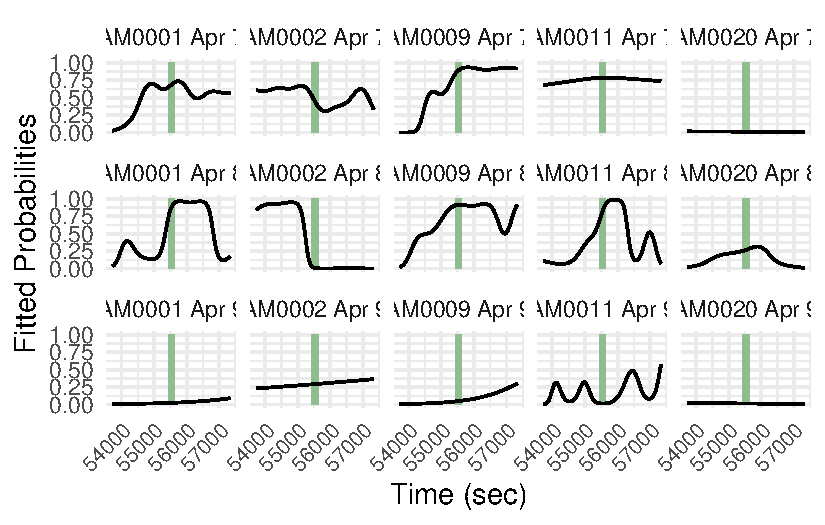
\includegraphics[keepaspectratio]{draft_paper_files/figure-pdf/unnamed-chunk-18-1.pdf}}

\linespread{2}

\section{Conclusion}\label{conclusion}

Altogether, the 2024 eclipse seemed to increase wildlife vocalizations,
but each individual species seem to respond in different ways. Spring
Peppers, see to drive the general, community-level pattern, with a peak
in vocalizations at totality, some other Anurans seem to share this
response. The birds responded more idosyncatrically, but some like the
Common Grackle, Rusty Blackbird, and Candian Goose, had a gap in calls
during totality with an heightened level of vocal activity around
totality. These differences in species-level responses may cause the
difference in vocalization pattern due to sight in the GAMM model, as
intersite differences species composition could result in the different
patterns seen on eclipse day. Models investingating specific species or
groups of related species may illucidate how their responsed drive the
overall community pattern across sites and the days studied.

Another key future step is to validate these data. The BirdNET output
includes a confidence score for each species prediction. We did not
discriminate based on this score as long as the confidence was greater
than 0.4. However, manual validation is required to know how to
threshold the data (to minimize misidentiifications), as well as
determine if each species requires a different threshold based on
detection difficulty (more cryptic species or more difficult for BirdNET
to identify). Without validation by experts, it remains unclear how
accurate BirdNET was in its predictions, and which data are
representitive of the actual vocalizations made by the wildlife
community we recorded.

The effectiveness of the GAMM model and our exploratory analysis
illustrate an increase in vocalization and differential species
responses to the 2024 total eclipse. With further investigation into
species-level responses and validation of the data, we can get an even
clearer understanding of how forest communities react to unexpected and
dramatic changes in light.




\end{document}
